\documentclass[12pt]{article}
\usepackage[spanish]{babel}
\usepackage[utf8]{inputenc}
\usepackage{graphicx}
\title{Modelo del Dominio}
\date{2025-05-26}
\usepackage[margin=1in]{geometry}
\begin{document}
    \begin{titlepage}
        \centering
        {\Large Universidad Central de Venezuela \par}
        \vspace{0.25cm}
        {\Large Facultad de Ciencias \par}
        \vfill
        {\LARGE Proyecto: Comedor Universitario \par}
        \vspace{0.25cm}
        {\bfseries\Huge Modelo del Dominio \par}
        \vfill
        \raggedright
        {\large Profesor: Marcel Castro \par}
        {\large Sección: C2 \par}
        \vspace{0.5cm}
        {\large Equipo \#4: \par}
        \begin{itemize}
            \item {\large Samantha Arellano} - C.I.30.830.771
            \item {\large Tobias Briceño} - C.I. 31.307.238
            \item {\large María Laura Reina} - C.I. 31.275.108
            \item {\large Victoria Ruza} - C.I. 30.946.460
        \end{itemize}
        \vspace{1cm}
        \centering
        {\large 26 de mayo del 2025 \par}
    \end{titlepage}

    \section{Diagrama de clases del dominio}
        \begin{center}
            \vfill
            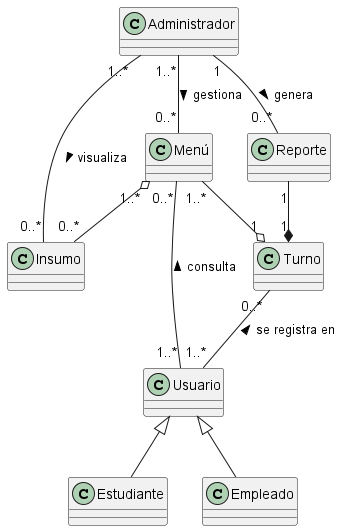
\includegraphics[width=10cm]{Partes/ModeloDominio.png}
            \vfill
        \end{center}

    \section{Glosario de términos:}
    \medskip
    \begin{itemize}
        \item \textbf{Estudiante:} Usuario del sistema que puede consultar menús, turnos y registrarse en estos para acceder al servicio del comedor.
        \item \textbf{Empleado:} Usuario del sistema que puede consultar menús, turnos y registrarse en estos para acceder al servicio del comedor.
        \item \textbf{Administrador:} Rol del sistema que permite gestionar y visualizar los menús semanales, insumos disponibles, registro de consumo diario y generar reportes correspondientes a cada turno.
        \item \textbf{Turno:} Horario en el que se ofrece el servicio del comedor universitario a estudiantes y empleados.
        \item \textbf{Insumo:} Materia prima utilizada en la preparación de los alimentos del comedor universitario que debe ser tomada en cuenta al gestionar los menús semanales.
        \item \textbf{Consumo Diario:} Registro de los alimentos consumidos por los usuarios del comedor universitario en un día específico, representado en los reportes de dicho día.
        \item \textbf{Reporte:} Documento generado por el administrador que permite analizar la demanda de un turno y planificar los recursos del comedor.
    \end{itemize}
    \newpage

    \section{Diagrama de contexto}

\end{document}